\section{Related Work}\marginnote{VTN}
    \begin{text}
    In this section, we would like to introduce two papers: \textit{Secure logistic regression Based on Homomorphic Encryption: Design and Evaluation} \cite{MiranKim2018}, and \textit{logistic regression model training based on the approximate homomorphic encryption} \cite{Kim2018}. Both of the papers present ways to implement logisctic regression based on the CKKS encryption scheme.
    \end{text}
    
    \subsection{Secure logistic regression Based on Homomorphic Encryption: Design and Evaluation}\marginnote{VTN}
    The authors adapted the CKKS encryption scheme which is optimized for real number computation. Notably, a least squares approximation of the logistic function is introduced to improve accuracy and efficiency.
    
    We know that the sigmoid function plays an important part in logistic regression data training using the gradient descent method. Despite the gradient descent can be used along with CKKS encryption scheme, there is still a computational difficulty during the implementation. The sigmoid function becomes that issue, because the CKKS can only evaluate the polynomial functions. Therefore, Taylor polynomials have been formulated as an approximate replacement of the sigmoid function. However, we found that even if the Taylor polynomial $T_9(x)$ is used, the accuracy is not enough; it is a local approximation near a certain point (see figure \ref{fig:approxsigmoid}a). 
    
    \begin{figure}[ht]
        \centering
        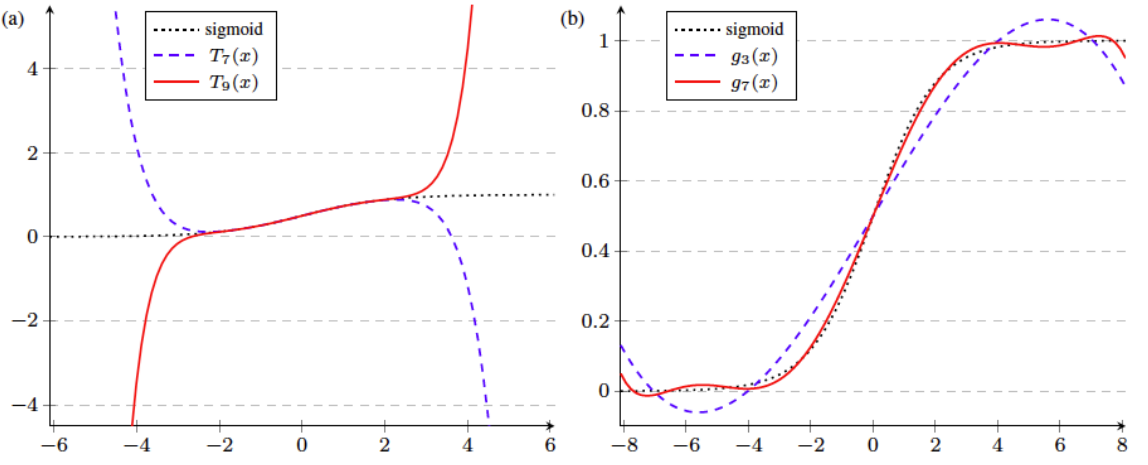
\includegraphics[width=1\linewidth]{images/Screenshot from 2021-10-03 23-12-29.png}
        $g_3(x)=0.5 + 1.20096 * (x/8) - 0.81562 * (x/8)^3$
        
        $g_7(x)=0.5 + 1.73496 * (x/8) - 4.19407 * (x/8)^3 + 5.43402 * (x/8)^5 - 2.50739 * (x/8)^7$
        \caption{Graphs of (a) sigmoid function and Taylor polynomials and (b) sigmoid function and least squares approximations. \cite{MiranKim2018}}
        \label{fig:approxsigmoid}
    \end{figure} 
    
    Due to limitation of the Taylor polynomial, Miran Kim at al. \cite{MiranKim2018} adopted a global approximation to minimize the the mean squared error which is defines by:
    $(1 / |I|) \int_{I}f(x)^2dx$, where $f(x)$ is an integrable function and $I$ is an interval. The least squares method is meant to produce a polynomial $g(x)$ of degree $d$ minimizing the mean squared error $(1 / |I|) \int_{I}(f(x) - g(x))^2dx$. The authors used degree 3 and 7 least squares approximation of the sigmoid function over the interval [-8,8] (see formulas in figure \ref{fig:approxsigmoid}). It has been proved that $g_3$ only needs a smaller depth for evaluation, while $g_7$ is more precise.

    \begin{text}
    In order to evaluate their method, five chosen datasets are described in table \ref{tab:miranDesOfData}. These single-binary-labeled datasets can be used to train binary classifiers, e.g., logistic regression. In table \ref{tab:miranCompare}, the final models of encrypted approach and encrypted logistic regression are compared. We see that the gaps between those models are not huge; therefore, the paper's approach is as good as the unencrypted logistic regression with the original sigmoid function. 
    \end{text}
    
    \begin{table}[ht]
        \centering
        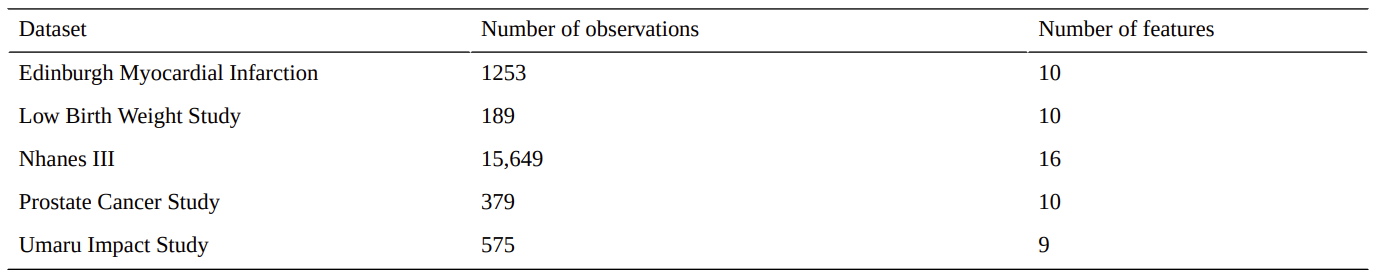
\includegraphics[width=1\linewidth]{images/Screenshot from 2021-10-03 23-53-36.png}
        \caption{Description of datasets. \cite{MiranKim2018}}
        \label{tab:miranDesOfData}
    \end{table} 
    
    \begin{table}[ht]
        \centering
        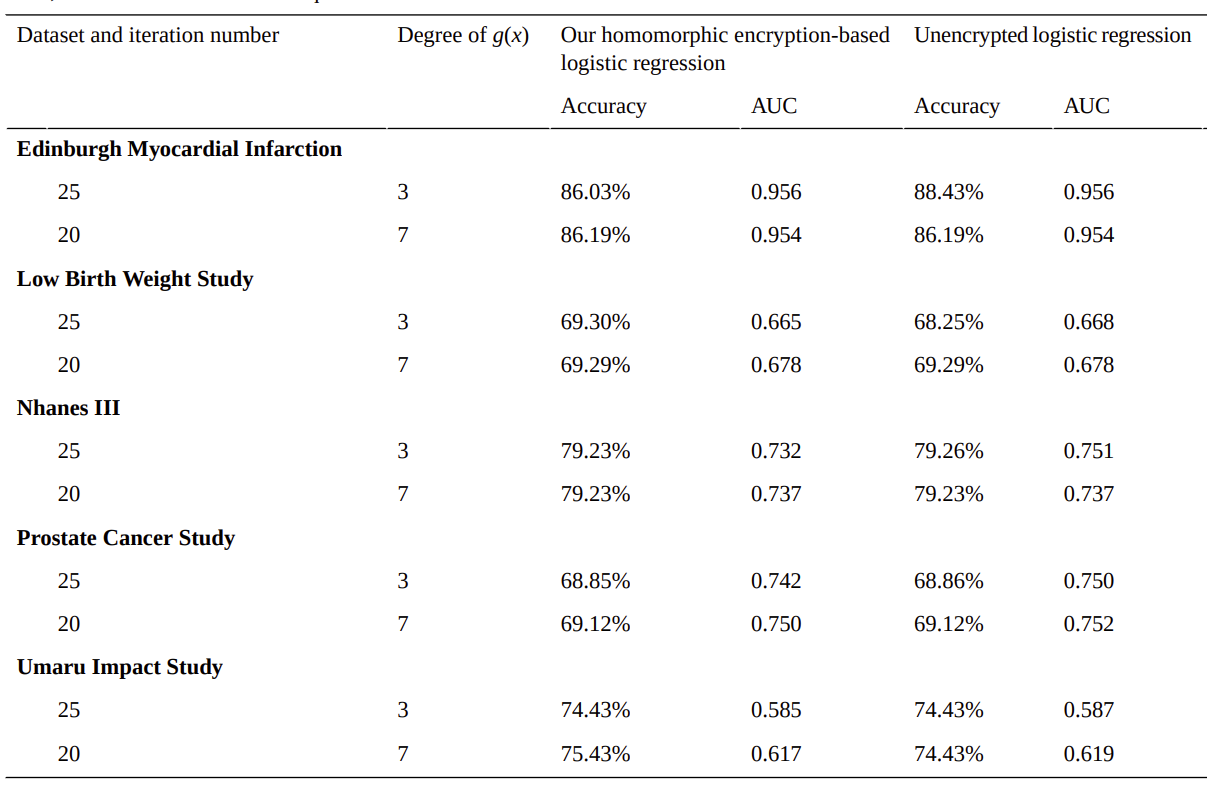
\includegraphics[width=1\linewidth]{images/Screenshot from 2021-10-04 00-12-26.png}
        \caption{Comparison of encrypted/unencrypted logistic regression. \cite{MiranKim2018}}
        \label{tab:miranCompare}
    \end{table} 
    
    \subsection{Logistic regression model training based on approximate homomorphic encryption}\marginnote{VTN}
    Similar to the papers of \cite{MiranKim2018}, \cite{Kim2018} also described a mean to train a logistic regression model without leaking any information by using the CKKS encryption scheme. Especially, they proposed a new encoding method to reduce the size of the encrypted database. In addition, adapting Nesterov's accelerated gradient descent helps to reduce the number of iterations as well as computational power while assuring the quality of final models.
    
    The Gradient Descent has an issue when dealing with the local minimas. If the learning rate is too low, we might stuck in a local minima; therefore, we cannot get to the global minima. Many gradient descent algorithms have been developed to overcome this problem, for example, momentum gradient descent. Nesterov Accelerated Gradient D`escent \cite{Nesterov} is a variant of momentum gradient descent. It applies moving average to the update vector, and calculate the gradient at this "look-ahead" position afterward. It is proved to give a better convergence of $O(1/t^2)$ after iterating $t$ steps theoretically as well as practically. The weight update equations of the Nesterov's accelerated gradient descent are shown in figure \ref{fig:nesteroveq}.
    
    \begin{figure}[ht]
        \centering
        $\theta^{(t+1)} \xleftarrow[]{} v^{(t)} - \alpha_t \cdot \nabla{J}(v^{(t)})$
    
        $v{(t+1)} \xleftarrow[]{} (1 - \gamma_t) * \theta^{(t+1)} + \gamma_t \cdot \theta^{(t)}$
        \caption{Equations of Nesterov Accelerated Gradient Descent. $0 < \gamma_t < 1$. $0 < \alpha_t < 1$}
        \label{fig:nesteroveq}
    \end{figure}
    
    In order to achieve an efficient computation, the authors pack all data points of a dataset into a single vector in row-by-row order. The concept is shown in figure \ref{fig:dataencodeconcept}; where each row represents one data point, $(f+1)$ is the number of features, and $n$ is the number of data points in the dataset. To evaluate gradient descent on the vector $w$, shifting operations of row and column vectors are needed. A shift algorithm \textit{Rot($w$, $r$)} can shift the encrypted vector $w$ by $r$ positions. For example, we get a new dataset $Z'$ (see figure \ref{fig:shiftedw}), if we do \textit{Rot($w$, $f+1$)} (which means we shift the vector $w$ by $(f+1)$ positions).
    
    \begin{figure}[ht]
	    \centering
	    \subfloat[][The dataset described as a matrix $Z$]{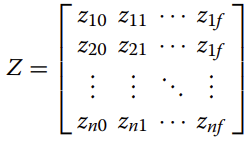
\includegraphics[width=0.3\linewidth]{images/Screenshot from 2021-10-04 01-48-54.png}\label{fig:matrixR}}\qquad
        \subfloat[][The matrix $Z$ is packed in a vector $w$]{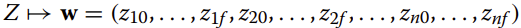
\includegraphics[width=0.47\linewidth]{images/Screenshot from 2021-10-04 01-49-05.png}\label{fig:vectorw}}
        \caption{Data encoding concept of paper \cite{Kim2018}} \label{fig:dataencodeconcept}
	\end{figure}
	
	\begin{figure}[ht]
        \centering
        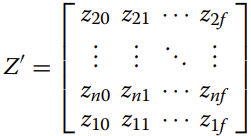
\includegraphics[width=0.3\linewidth]{images/Screenshot from 2021-10-04 02-04-49.png}
        \caption{New matrix $Z'$ corresponding to the shifted vector $w'$. Where $w'$ = \textit{Rot($w$, $f+1$)} \cite{Kim2018}}
        \label{fig:shiftedw}
    \end{figure} 
    
    Applying the Nesterov Accelerated Gradient Descent \cite{Nesterov} and the data packing approach above, we achieve similar output models as the approach described in \cite{MiranKim2018} with much less runtimes and less allocated memory. The results are shown in the table \ref{fig:comparetable}.
    
    \begin{table}
    \resizebox{\textwidth}{!}{\begin{tabular}{ c c c c c c c c c c c }
    \hline
    Dataset & Sample num & Feature num & Method & deg $g$ & Iter num & Enc time & Learn time & Storage & Accuracy & AUC\\
    \hline
    \multirow{3}{4em}{Edinburgh} & \multirow{3}{4em}{1253} & \multirow{3}{4em}{9} & \cite{Kim2018} & 5 & 7 & 2s & 3.6 min & 0.02 GB & 91.04\% & 0.958  \\ 
    &&& \cite{MiranKim2018} & 3 & 25 & 12s & 114 min & 0.69 GB & 86.03\% & 0.956 \\ 
    &&& \cite{MiranKim2018} & 7 & 20 & 12s & 114 min & 0.71 GB & 86.19\% & 0.954 \\ 
    \multirow{3}{4em}{lbw} & \multirow{3}{4em}{189} & \multirow{3}{4em}{9} & \cite{Kim2018} & 5 & 7 & 2s & 3.3 min & 0.02 GB & 69.19\% & 0.689  \\ 
    &&& \cite{MiranKim2018} & 3 & 25 & 11s & 99 min & 0.67 GB & 69.30\% & 0.665 \\ 
    &&& \cite{MiranKim2018} & 7 & 20 & 11s & 86 min & 0.70 GB & 69.29\% & 0.678 \\ 
    \multirow{3}{4em}{nhanes3} & \multirow{3}{4em}{15649} & \multirow{3}{4em}{15} & \cite{Kim2018} & 5 & 7 & 14s & 7.3 min & 0.16 GB & 79.22\% & 0.717  \\ 
    &&& \cite{MiranKim2018} & 3 & 25 & 21s & 235 min & 1.15 GB & 79.23\% & 0.732 \\ 
    &&& \cite{MiranKim2018} & 7 & 20 & 21s & 208 min & 1.17 GB & 79.23\% & 0.737 \\ 
    \multirow{3}{4em}{pcs} & \multirow{3}{4em}{379} & \multirow{3}{4em}{9} & \cite{Kim2018} & 5 & 7 & 2s & 3.5 min & 0.02 GB & 68.27\% & 0.740  \\ 
    &&& \cite{MiranKim2018} & 3 & 25 & 11s & 103 min & 0.68 GB & 68.85\% & 0.742 \\ 
    &&& \cite{MiranKim2018} & 7 & 20 & 11s & 97 min & 0.70 GB & 69.12\% & 0.750 \\ 
    \multirow{3}{4em}{uis} & \multirow{3}{4em}{575} & \multirow{3}{4em}{8} & \cite{Kim2018} & 5 & 7 & 2s & 3.5 min & 0.02 GB & 74.44\% & 0.603  \\ 
    &&& \cite{MiranKim2018} & 3 & 25 & 10s & 104 min & 0.61 GB & 74.43\% & 0.585 \\ 
    &&& \cite{MiranKim2018} & 7 & 20 & 10s & 96 min & 0.63 GB & 75.43\% & 0.617 \\ 
    \hline
    \end{tabular}}
    \caption{Implementation results for 5 datasets with 5-fold CV \cite{Kim2018}}
    \label{fig:comparetable}
    \end{table}